\documentclass{article}

%%%%%%%%%%%%%%%%%%%%%%%%%%%%%%%%%% Maths %%%%%%%%%%%%%%%%%%%%%%%%%%%%
\usepackage{amsmath}

%%%%%%%%%%%%%%%%%%%%%%%%%%%%%%%%%% referencing %%%%%%%%%%%%%%%%%%%%%%%%%%%%%%%%%%
\usepackage{natbib}
\usepackage{hyperref}
\usepackage{todonotes}

%%%%%%%%%%%%%%%%%%%%%%%%%%%%%%%%%% figure and table %%%%%%%%%%%%%%%%%%%%%%%%%%%%%%%%%%
\usepackage{graphicx}

%%%%%%%%%%%%%%%%%%%%%%%%%%%%%%%%%% layout %%%%%%%%%%%%%%%%%%%%%%%%%%%%%%%%%%
\usepackage{setspace}
\linespread{1.5}
\usepackage{fullpage}


\usepackage{subfig}

\begin{document}

\title{The rate and structure of mixed infections in global populations of {\it Plasmodium} malaria}
\date{}
\maketitle
{}
\listoftodos
{}

\todo{Afflictions}

\todo{running title}

\todo{keywords}

\begin{abstract}
  \todo{abstract}
The extent to which individuals infected with malaria pathogens of the genus {\it Plasmodium} carry multiple, genetically distinct strains both reflects local epidemiological processes and can influence the nature and severity of disease.  Large-scale genome sequencing projects of malaria pathogens have the potential to provide high resolution information about the rate and structure of mixed infections, but current analytical approaches often fail to fully capture the diversity and relatedness structure of strains present.  Here, we introduce an enhanced method for deconvolution of mixed infections that identifies the number of strains and patterns of identity by descent between them.  We apply the approach to XXX samples of {\it P. falciparum} from XXX populations and XXX samples of {\it P. vivax} from across XXX populations.  Rates of mixed infection vary from XX\% to XX\%, with up to XX\% of individuals carrying at least three strains in XXX.  In between XX\% and XX\% of cases we find evidence for sibling strains, likely arising from a single bite by a multiply-infected mosquito.  The proportion of mixed infections with sibling strains is remarkably constant across species and populations.  Our findings suggest that the rate and relatedness structure of mixed infections will be valuable metrics in characterising malaria epidemiology and mapping changes over space and time.
\end{abstract}

\section{INTRODUCTION}
1. Why mixed infection is relevant to biology and epidemiology.

Humans with P. falciparum malaria often have mixed infections, i.e. they carry a mixture of genetically different parasites of the same species.  Sometimes this is the result of multiple mosquito bites, particularly in geographical locations with high levels of malaria transmission.  On other occasions it is the result of a single mosquito transmitting a genetic mixture of parasites from one person to another.  This is of considerable biological interest because the parasites undergo sexual recombination within the mosquito, i.e. transmission of mixed infections enables new genetic forms to be generated by sexual recombination within the parasite population.

Genetic analysis of mixed infections is therefore a central problem in P. falciparum population biology.  It is also a practical problem, because mixed infections make it difficult to analyse genome variation within a sample. Current approaches are largely based on genotyping multiple loci (e.g. SNPs) to identify heterozygous genotypes and to measure their allelic proportions, from which it is possible to estimate the complexity of infection (COI) and a coefficient of inbreeding (Fws) within a sample [Manske et al., 2012], [Auburn et al., 2012], [Galinsky et al., 2015].  Such metrics are useful for comparing levels of mixed infection between different locations, and for investigating correlation with transmission intensity and other epidemiological variables, but they do not capture the underlying genetic architecture of an individual mixed infection.

2. Prior art – what have others found about rates of mixed infection?

3. Previous work on DEploid – method for deconvolution of mixed infections, using a reference panel.
Because of the difficulty of analysing samples with mixed infection, most studies of P. falciparum have focused on samples harbouring a single dominant strain.

4. However, we observed that in cases with inbreeding we sometimes failed to separate related strains.

5. Here we develop an enhanced version that models IBD patterns and incorporates into strategy (first estimate IBD and no. strains, then use reference panel version).

6. Apply to 2 large data sets.

7. Findings relevant to efforts to use genomic data to develop genomic predictors of epidemiological parameters.

\section{Method outline and validation}

1. Overview of approach.  Figure 1a, schematic of approach.
\begin{figure}
  \centering{}
  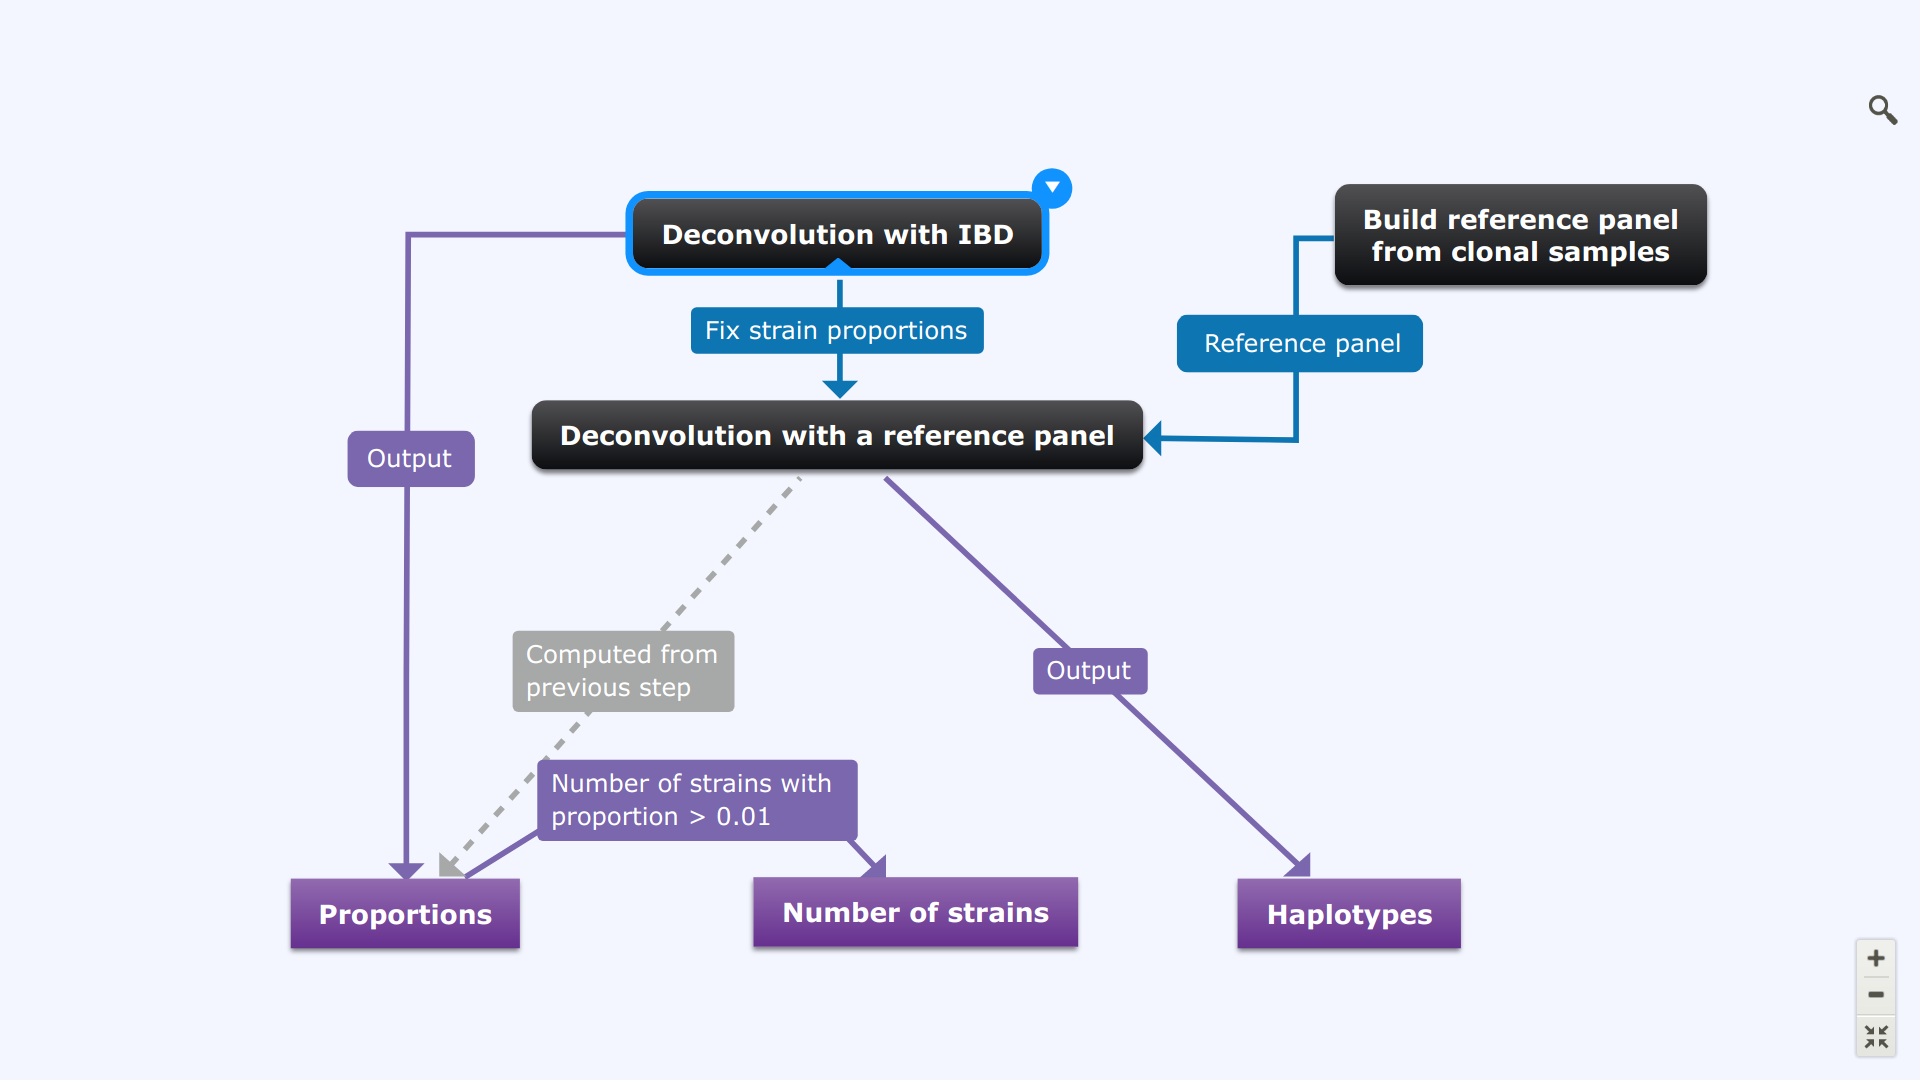
\includegraphics[width=0.8\textwidth]{figures/scheme.png}
  \caption{Schematic approach. Black box indicates when DEploid is used. Purple box indicates output.}\label{fig:scheme}
\end{figure}

2. Joint estimation of IBD, strains and proportions.  Details in SOM.  Figure 1b.  Example deconvolution in real data showing IBD transitions.

3. Validation through empirical data analysis and simulation.  Figure 2 showing simulation results.  Supplementary Figure 1 showing effective k under DEploid with and without IBD.
\begin{figure}
  \centering{}
  \subfloat[][]{
  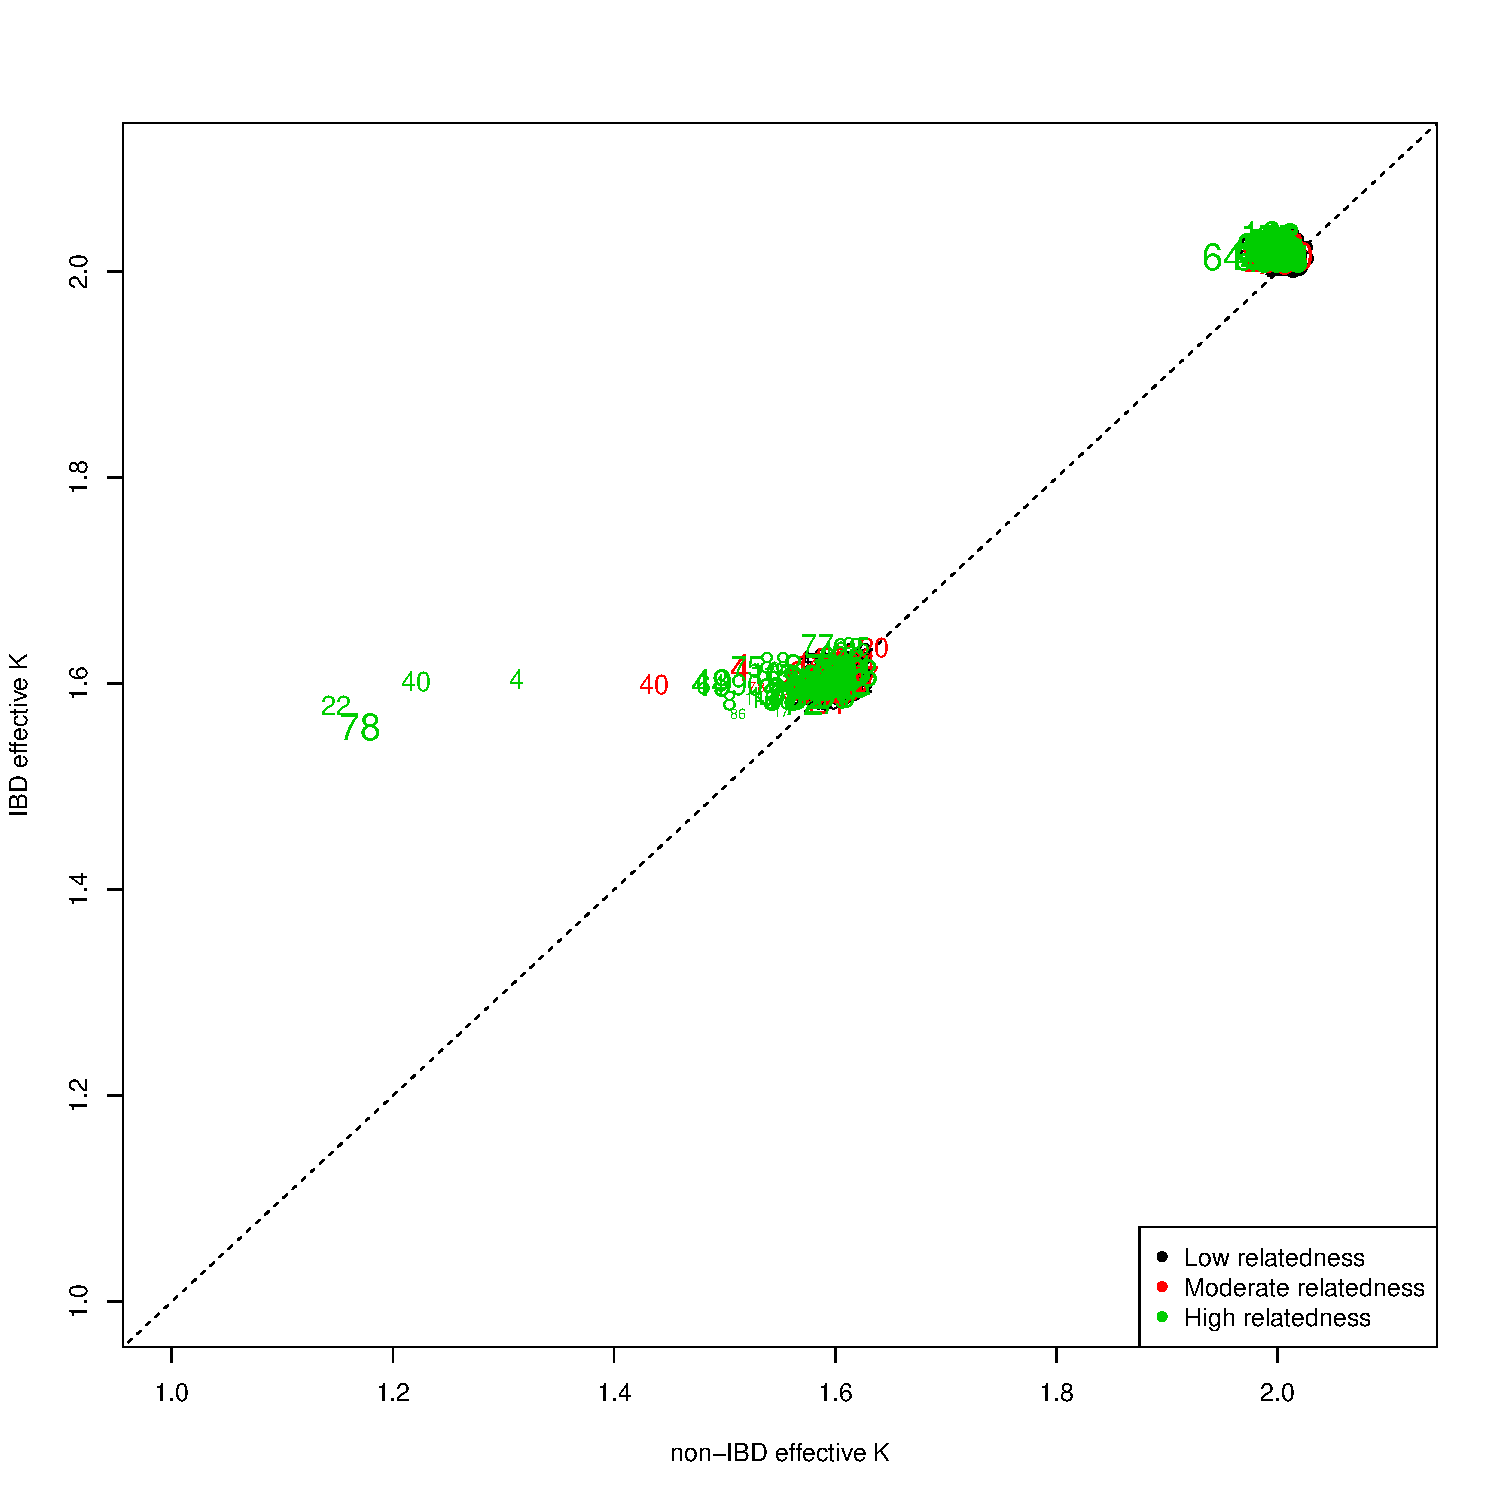
\includegraphics[width = 0.45\textwidth]{figures/diagnositicPlot_of_effK_final.pdf}
  }
  \subfloat[][]{
  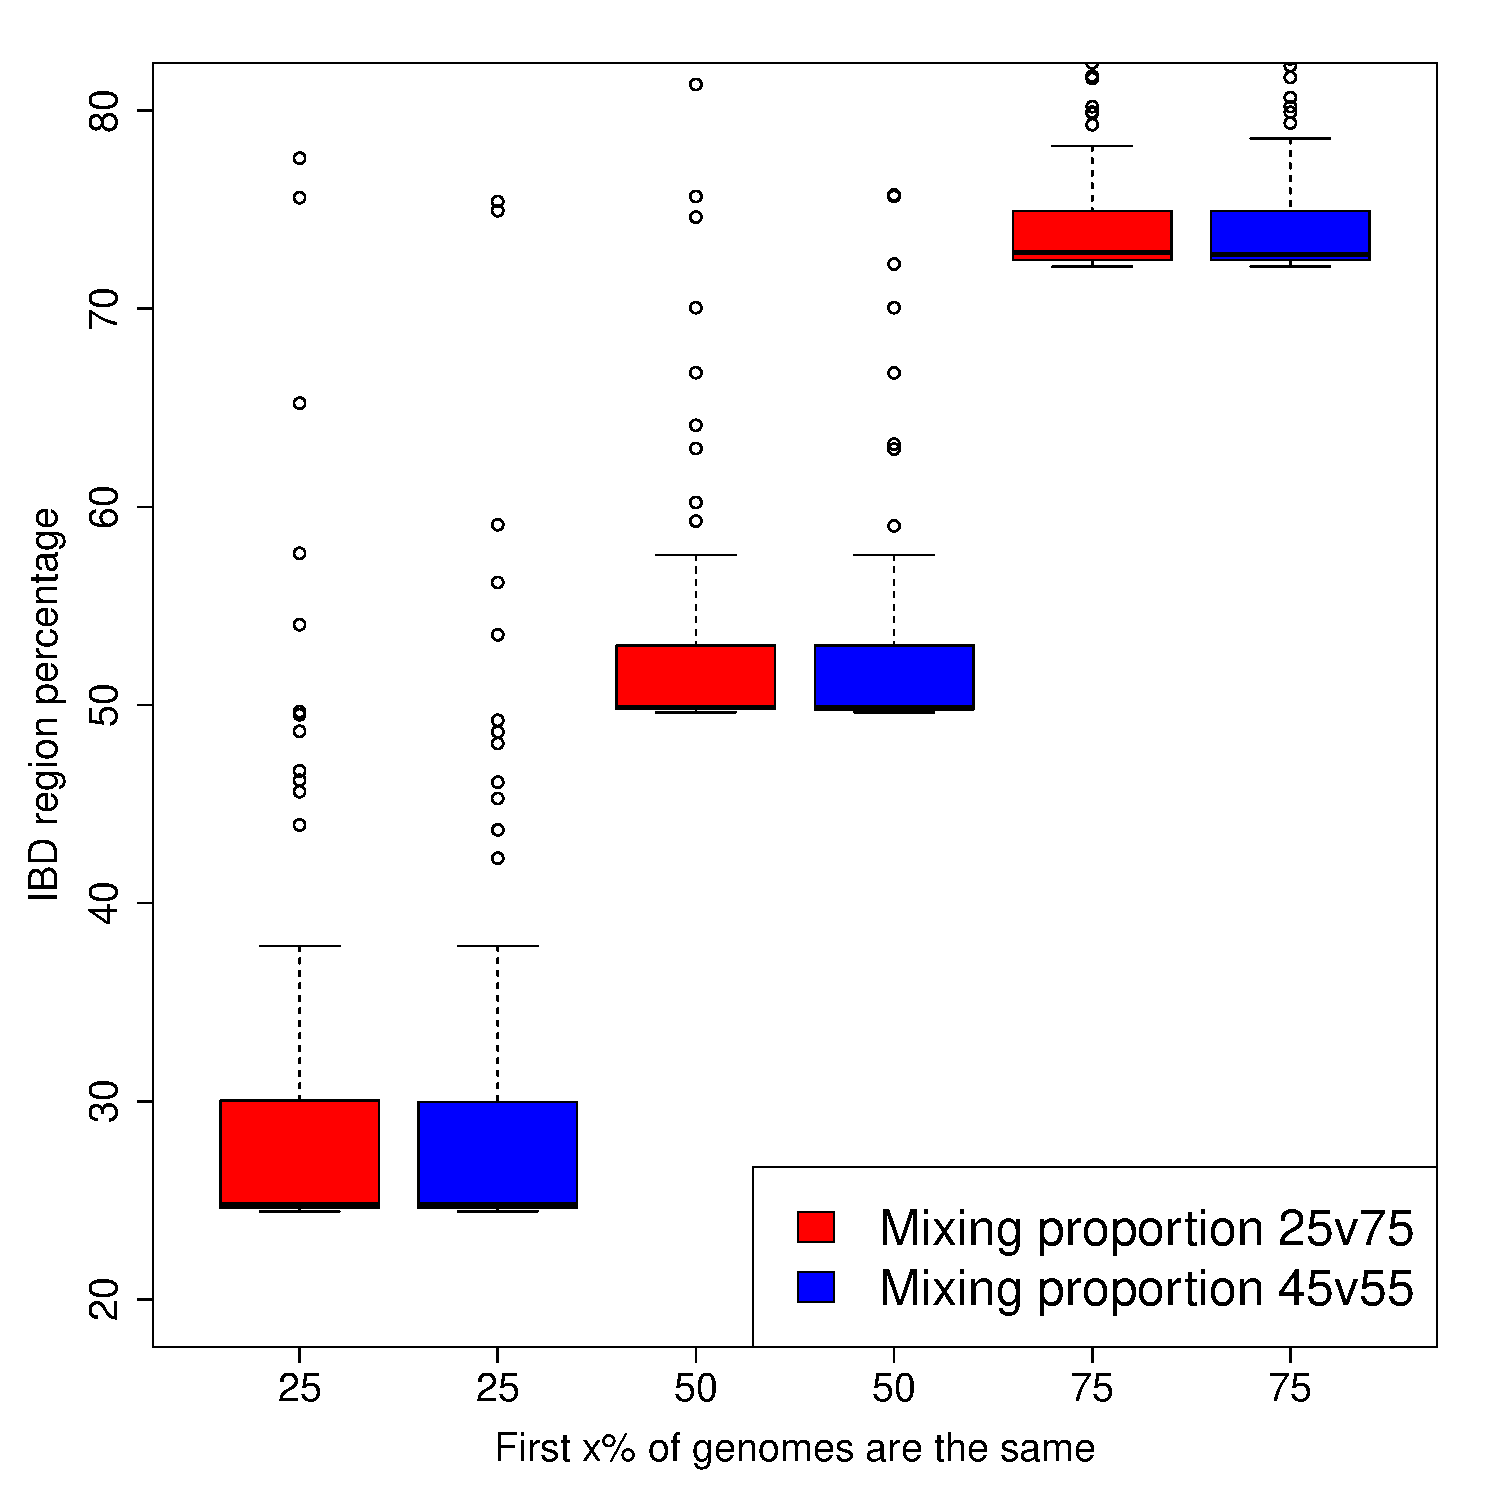
\includegraphics[width = 0.45\textwidth]{figures/IBDprobs.pdf}
  }
  \caption{Simulation results}
\end{figure}


\section{Application to Pf and Pv data}
1. Data source and preparation (i.e. cleaning).  Supplementary Figure 2 on importance of strong variant filtering.

2. Summary of findings within Pf and Pv. Figure 3: Rates of co-infection by geography and species.

3. Summary of findings about relatedness within mixed infections.  Figure 4.  Relatedness structure histogram showing peaks at 0.25, 0.5, etc. and relationship between mixed infection rate and sib-strain.

4. Simulation results to analyse the relationship between prevalence, mixed infection rate and sib-strain rate.  Figure 5 summarising simulations.

\section{Discussion}

1. Recap of main findings.

2. Relationship of mixed infection to prevalence v population size from simulations and interpretation of empirical data in the light of this.

3. Interpretation of within and between sample relatedness – does it reflect some feature of underlying biology?

4. Directions for integrating genomic data into efforts to map spatial and temporal changes in prevalence.





\section{ACKNOWLEDGMENTS}
We thank the Pf3k consortium for valuable insights. The project is funded by the Wellcome Trust grant [100956/Z/13/Z] to GM.

\section{DISCLOSURE DECLARATION}
None declared.


\begin{thebibliography}{}

\bibitem[\protect\citeauthoryear{Browning and Browning}{Browning and
  Browning}{2007}]{Browning2007}
Browning, S.~R. and B.~L. Browning (2007)
\newblock Rapid and accurate haplotype phasing and missing-data inference for
  whole-genome association studies by use of localised haplotype clustering.
\newblock {\em Am. J. Hum. Genet.\/}~{\em 81\/}(5), 1084--1097.

\bibitem[\protect\citeauthoryear{Neafsey}{Neafsey}{2012}]{Neafsey2012}
Neafsey, D. {\em et al}.(2012)
\newblock The malaria parasite {\it Plasmodium vivax} exhibits greater genetic diversity than {\it Plasmodium falciparum}.
\newblock {\em Nature Genetics\/}~{\em 44\/}(9), 1046--1052.

\bibitem[\protect\citeauthoryear{Wegmann}{Wegmann}{2011}]{Wegmann2011}
Wegmann, D. {\em et al}.(2011)
\newblock Recombination rates in admixed individuals identified by ancestry-based inference.
\newblock {\em Nature Genetics\/}~{\em 43\/}, 847--894.

\bibitem[\protect\citeauthoryear{Hinch}{Hinch}{2011}]{Hinch2011}
Hinch, A.G. {\em et al}. (2011))
\newblock The landscape of recombination in African Americans.
\newblock {\em Nature\/}~{\em 476}, 170--175.

\bibitem[\protect\citeauthoryear{Henden}{Henden}{2016}]{Henden2016}
Henden, L. {\em et al}. (2016))
\newblock Detecting selection signals in {\it Plasmodium falciparum} using identity-by-descent analysis,
\newblock {\em bioRxiv.\/}, 088039.


\bibitem[\protect\citeauthoryear{Mu}{Mu}{2005}]{Mu2005}
Mu, J. {\em et al}. (2005)
\newblock Recombination Hotspots and Population Structure in {\it Plasmodium falciparum}.
\newblock {\em PLOS Biology.\/}~{\em 3}, e335.


\bibitem[\protect\citeauthoryear{Lopez}{Lopez}{2012}]{Lopez2012}
Lopez A. {\em et al}. (2012)
\newblock Genetic diversity of {\it Plasmodium vivax} and {\it Plasmodium falciparum} in Honduras.
\newblock {\em Malaria Journal.\/}~{\em 11}, 391.

\bibitem[\protect\citeauthoryear{Jiang}{Jiang}{2011}]{Jiang2011}
Jiang, H. {\em et al}. (2011)
\newblock High recombination rates and hotspots in a {\it Plasmodium falciparum} genetic cross.
\newblock {\em Genome Biology.\/}~{\em 12}, R33.


\bibitem[\protect\citeauthoryear{Miles, Iqbal, Vauterin, Pearson, Campino,
  Theron, Gould, Mead, Drury, O{\textquoteright}Brien, Ruano~Rubio, MacInnis,
  Mwangi, Samarakoon, Ranford-Cartwright, Ferdig, Hayton, Su, Wellems, Rayner,
  McVean, and Kwiatkowski}{Miles et~al.}{2016}]{Miles2016}
Miles, A. {\em et al}. (2015)
\newblock Indels, structural variation, and recombination drive genomic diversity in {\it Plasmodium falciparum}.
\newblock {\em Genome Res.\/}~{\em26\/}, 1288--1299.

\bibitem[\protect\citeauthoryear{O'Brien}{O'Brien et~al.}{2016}]{Jack2016}
O'Brien D,J. {\em et al}. (2016)
\newblock Inferring Strain Mixture within Clinical {\em Plasmodium falciparum} Isolates from Genomic Sequence Data.
\newblock {\em PLoS Comput. Biol.\/}~{\em 12\/}(6): e1004824.

\bibitem[\protect\citeauthoryear{O'Brien}{O'Brien et~al.}{2015}]{Jack2016Inbreeding}
O'Brien D,J. {\em et al}. (2016)
\newblock Approaches to estimating inbreeding coefficients in clinical isolates of {\it Plasmodium falciparum} from genomic sequence data.
\newblock {\em Malaria Journal\/}~{\em 15}:473.


\bibitem[\protect\citeauthoryear{Pearson, Amato, Auburn, Miotto,
  Almagro-Garcia, Amaratunga, Suon, Mao, Noviyanti, Trimarsanto, Marfurt,
  Anstey, William, Boni, Dolecek, Tran, White, Michon, Siba, Tavul, Harrison,
  Barry, Mueller, Ferreira, Karunaweera, Randrianarivelojosia, Gao, Hubbart,
  Hart, Jeffery, Drury, Mead, Kekre, Campino, Manske, Cornelius, MacInnis,
  Rockett, Miles, Rayner, Fairhurst, Nosten, Price, and Kwiatkowski}{Pearson
  et~al.}{2016}]{Pearson2016}
Pearson, R.~D. {\em et al}. (2016)
\newblock {Genomic analysis of local variation and recent evolution in {\it Plasmodium vivax}}.
\newblock {\em Nat. Genet.\/}~{\em 48}, 959--964.


\bibitem[\protect\citeauthoryear{Rutledge}{Rutledge et~al.}{2017}]{Rutledge2017}
Rutledge. G. G., {\em et al}. (2017)
\newblock {\it Plasmodium} malariae and P. ovale genomes provide insights into malaria parasite evolution
\newblock {\em Nature.\/}~{\em 542}, 101--104.


\bibitem[\protect\citeauthoryear{Pf3k}{Pf3k}{2016}]{Pf3k2016}
The Pf3k Project: pilot data release 5 (2016)
\newblock {www.malariagen.net/data/pf3k-5} [accessed 1 June 2016]


\bibitem[\protect\citeauthoryear{WHO}{WHO}{2016}]{WHO2016}
WHO. (2016)
\newblock {World Malaria Report 2015}.
\newblock {\em World Health Organization\/}.

\bibitem[\protect\citeauthoryear{Zhu, Garcia, McVean}{Zhu et~al.}{2017}]{Zhu2017}
Zhu, J. S.\, J. A. Garcia\, G. McVean. (2017)
\newblock {Deconvoluting multiple infections in {\it Plasmodium falciparum} from high throughput sequencing data}.
\newblock {\em bioRxiv\/}~{\em \/}099499. doi: https://doi.org/10.1101/099499

\end{thebibliography}

\end{document}
